\subsubsection{Seguidor de línea}

A pesar de ser una herramienta fundamental para estimar la posición y orientación del robot, la odometría está sujeta a errores. Por lo que se hace necesario contar con un mecanismo adicional para poder detectar desviaciones en la trayectoria. Para esto se propone un seguidor de línea colocado de modo que el robot pueda detectar cuando se sale por fuera de las trayectorias determinadas por las líneas.

Un seguidor de línea es un sistema basado en sensores que detectan marcas en el entorno y utilizan esta información para ajustar la trayectoria del robot de manera automática.

La implementación de un seguidor de línea en robots omnidireccionales ofrece varias ventajas. En primer lugar, permite corregir desviaciones causadas por errores acumulativos en la odometría, ya que los sensores del seguidor de línea proporcionan información directa sobre la posición del robot respecto a la línea de referencia y en tiempo real.


\paragraph{Elección de método de seguimiento} \mbox{} \vspace{8pt}

Existen distintas técnicas para detectar una linea que un robot puede seguir. \\

\textbf{Seguidor de Línea Ultrasónico} \mbox{} \vspace{6pt} \\
Utiliza sensores ultrasónicos para detectar la presencia de una línea guía de la cual el robot debe mantenerse equidistante. Estos sensores emiten ondas sonoras de alta frecuencia y miden el tiempo que estas tardan en reflejarse al encontrar una superficie, lo que permite al robot seguir una trayectoria de manera precisa.

Entre sus ventajas, destaca su robustez, ya que no se ven afectados por factores como la suciedad o la iluminación, y su precisión, al detectar con alta exactitud la distancia hacia la línea guía. Sin embargo, estos sistemas presentan algunas desventajas, como la mayor complejidad y costo asociados con los sensores ultrasónicos, así como un alcance limitado en comparación con otros tipos de sensores. \cite{venkateshrfidultrasonic} \cite{aungultrasonic} \\


\textbf{Seguidor de Línea por Cámara} \mbox{} \vspace{6pt} \\
El seguidor de línea por cámara utiliza cámaras y algoritmos de procesamiento de imágenes para identificar y seguir líneas en el suelo de manera eficiente. Estas tecnologías permiten que el sistema sea altamente versátil, adaptándose a distintos tipos de líneas y patrones, al tiempo que proporcionan información adicional sobre el entorno que rodea al robot.

No obstante, esta solución presenta ciertos desafíos. Por un lado, requiere algoritmos avanzados de procesamiento de imágenes, lo que puede complicar su implementación. Por otro, su desempeño puede verse afectado por cambios en las condiciones de iluminación, lo que limita su eficacia en entornos variables. \cite{inianlinefollowcamera} \\


\textbf{Seguidor de Línea Ópticos} \mbox{} \vspace{6pt} \\
Los seguidores de línea ópticos son una de las implementaciones más comunes, ya que emplean sensores ópticos para detectar el contraste entre una línea dibujada en el suelo, generalmente negra, y el fondo, que suele ser blanco. Sensores como los fotodiodos o fototransistores envían señales al controlador del robot, permitiéndole ajustar su trayectoria para mantenerse sobre la línea. Entre las opciones disponibles, las versiones láser o infrarrojas son las más utilizadas.

Este sistema tiene como principales ventajas su simplicidad y bajo costo, ya que es relativamente sencillo de implementar, así como la amplia disponibilidad de estos dispositivos en el mercado. Sin embargo, también presenta algunas desventajas. Su rendimiento puede verse afectado por factores ambientales como la iluminación variable, el polvo, la suciedad y las superficies reflectantes, además de mostrar menor precisión en superficies no uniformes. Adicionalmente, las líneas pintadas en el suelo pueden desgastarse con el tiempo, requiriendo mantenimiento constante. \\


\textbf{Seguidor de Línea Magnético} \mbox{} \vspace{6pt} \\
El seguidor de línea magnético utiliza bandas magnéticas adheridas al suelo o a una pared, las cuales son detectadas por sensores magnéticos. Estos sensores identifican cambios en el campo magnético, permitiendo al robot seguir con precisión la trayectoria marcada por las bandas magnéticas.

Entre las ventajas de este sistema se encuentra su inmunidad al entorno, ya que no es afectado por factores como la suciedad, el polvo, la iluminación variable o las superficies reflectantes. Además, las bandas magnéticas destacan por su durabilidad, resistiendo condiciones ambientales adversas y requiriendo poco mantenimiento, mientras que ofrecen alta precisión en la navegación, especialmente en entornos industriales. Sin embargo, este sistema también presenta desventajas, como el mayor costo asociado a los sensores y bandas magnéticas en comparación con sistemas ópticos, así como el tiempo y esfuerzo necesarios para instalar dichas bandas. \\


\textbf{Seguidor de Línea con Etiquetas RFID} \mbox{} \vspace{6pt} \\
El seguidor de línea con etiquetas RFID utiliza etiquetas RFID incrustadas en el suelo o las paredes, junto con lectores RFID instalados en el robot, para detectar la presencia y posición de dichas etiquetas. Este sistema permite al robot interpretar su entorno de forma más inteligente al acceder a la información adicional almacenada en las etiquetas.

Entre las ventajas de este enfoque se encuentran la capacidad de las etiquetas RFID para proporcionar información adicional que facilita una navegación más eficiente, su inmunidad a factores ambientales como suciedad, polvo, variaciones en la iluminación o superficies reflectantes, y su flexibilidad para diseñar trayectorias más complejas y adaptativas. Sin embargo, presenta algunas desventajas, como el alto costo asociado a los sistemas RFID debido al precio tanto de los lectores como de las etiquetas, así como la mayor complejidad requerida para su implementación y configuración en comparación con otros sistemas. \cite{venkateshrfidultrasonic} \\


Al evaluar las diferentes alternativas, optamos por un seguidor de línea magnético dado que es el que mejor se adapta a los requerimientos de funcionamiento del robot. Una de las principales ventajas es la inmunidad a las condiciones del entorno y su relativo bajo costo. No se ven afectados por elementos que pueden interferir con los sensores ópticos, como la suciedad, el polvo, la iluminación variable, superficies reflectantes o las sombras. Esta característica aumenta la robustez del sistema en entornos industriales o comerciales donde las condiciones pueden ser menos que ideales.

Otra ventaja importante es la durabilidad y el mantenimiento reducido. Las bandas magnéticas son resistentes al desgaste y pueden soportar condiciones ambientales variables, reduciendo la necesidad de mantenimiento frecuente y aumenta la vida útil del sistema. En comparación, en caso de un sensor óptico, las líneas pintadas o adhesivas pueden desgastarse con el tiempo y requerir repintado o reemplazo periódico. Además, se pueden colocar de manera discreta dado que no es necesario que sean visibles.


\paragraph{Implementación} \mbox{} \vspace{8pt}

Se hizo una pieza impresa en 3D y se colocaron los sensores una determinada distancia entre sí obtenida experimentalmente. El arreglo de sensores Hall se coloca en el frente del robot y se mejoró la pista adhiriendo los imanes.

El procedimiento para compensar el robot se basa en que al tocar un imán de los extremos significa que existe una determinada distancia angular que difiere del vector de dirección deseado. Se representa esta distancia mediante $d_{r\theta}$:

\begin{figure}[H]
    \centering
    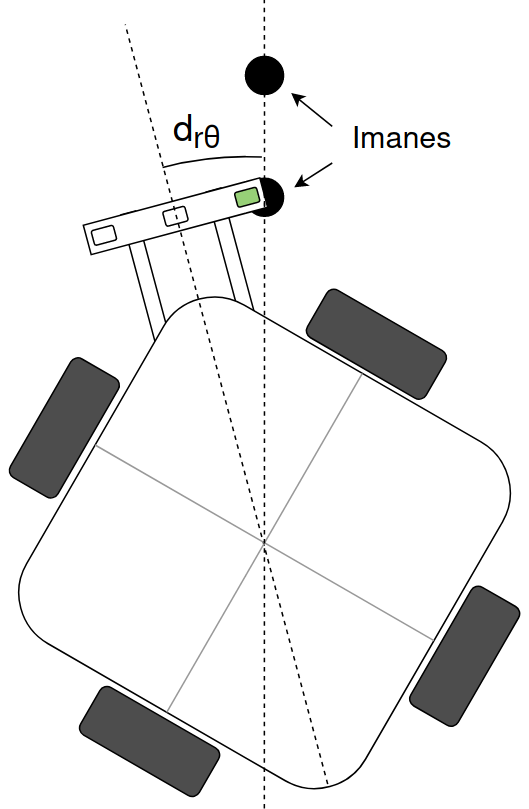
\includegraphics[width=0.4\linewidth]{images/robot_desplazamiento_angular_toca_iman.png}
    \caption{Escenario de detección de un imán}
    \label{fig:deteccionimanrobot}
\end{figure}

El enfoque propuesto es el de tener un acumulador que mide la distancia recorrida angularmente y ajusta la velocidad rotacional para compensar el desfase. Cada vez que se detecta un imán se suma o se resta un determinado valor de distancia angular de modo que el controlador intente llevarla a 0 nuevamente. Por ejemplo, si el robot detecta un desplazamiento hacia la derecha, se aumenta la velocidad rotacional hacia la izquierda.

El algoritmo de control opera de la siguiente manera:

\begin{enumerate}
    \item Los sensores magnéticos son monitoreados continuamente para detectar la presencia de imanes. Cada vez que se detecta un imán en alguno de los extremos, se actualiza un acumulador de distancia angular recorrida sumando o restando un valor determinado. Este valor depende de la distancia de los sensores al centro del robot y de la distancia entre los mismos.

    \item El objetivo es que el acumulador se mantenga en cero, lo que indicaría que el robot sigue la dirección de la trayectoria. El sistema de control ajusta las velocidades de las ruedas del robot en tiempo real en función al desplazamiento angular detectado.    
\end{enumerate}

Al realizar las pruebas, se lanzó al robot en distintas circunstancias, comenzando alineado con los imanes y comenzando con una desviación detectable. A medida que se avanzaron los ensayos se fue iterando sobre los coeficientes del seguidor de línea para compensar el error.

En una primera instancia, la implementación de la corrección del desplazamiento angular estaba dado por una velocidad fija. En las sucesivas experiencias, notamos que el robot a bajas velocidades se comportaba de un modo esperado y que a medida que se incrementaba la velocidad era menos estable. Es por ello que se cambió la velocidad constante por una que sea variable según la velocidad lineal del robot, es decir, ahora la compensación es adaptativa. De modo que a mayor velocidad lineal, mayor velocidad rotacional para realizar la compensación. Esto se debe a la inercia del robot, implicando que a mayor velocidad requiere mayor compensación para vencer el momento del mismo.

En la Figura \ref{fig:diagsecuencialinefollowmodcin} se detalla un diagrama de secuencia del funcionamiento del modelo cinemático compensado con el seguidor de línea.

\begin{figure}[H]
    \centering
    \hspace*{-1.25cm}
    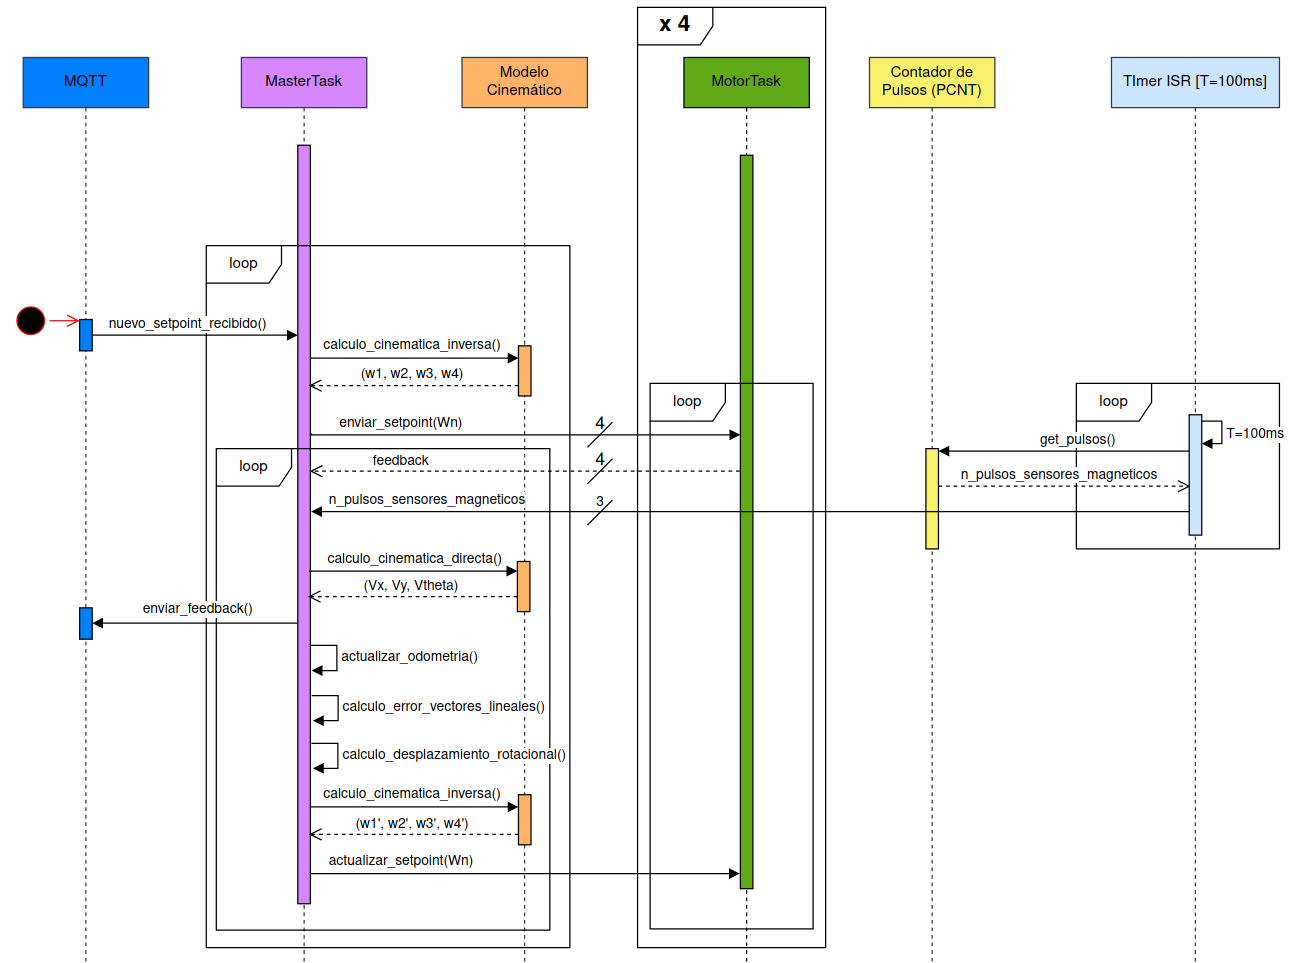
\includegraphics[width=1.2\linewidth]{images/diag_secuencia_seguidor_linea_magnetica_modelo_cinem_compensado.png}
    \caption{Diagrama de secuencia del seguidor de linea con el Modelo Cinemático}
    \label{fig:diagsecuencialinefollowmodcin}
\end{figure}

